\chapter{Implementasi dan Pengujian}
\label{chap:implementasi}

Pada bab ini terdapat dua bagian, yaitu Implementasi Perangkat Lunak dan Pengujian Perangkat Lunak. Bagian implementasi akan menjelaskan tentang lingkungan pengembangan perangkat lunak dan hasil implementasi. Bagian pengujian akan berisi hasil pengujian fungsional terhadap perangkat lunak yang telah dibangun.

\section{Implementasi}
\label{sec:implementasi}

\subsection{Implementasi}
Implementasi dilakukan dengan menggunakan laptop dengan spesifikasi sebagai berikut :
\begin{enumerate}
	\item \textit{Processor} : Intel(R) Core(TM) i5-4200U CPU @ 1.60GHz 2.30GHz
	\item RAM : 4.00 GB
	\item Sistem Operasi : Windows 10 Pro 64-bit
	\item Versi Netbeans : 8.0.2
\end{enumerate}

\subsection{Hasil Implementasi}
\begin{enumerate}
	\item Tampilan Bobot Ketetanggaan
	
	
	Seperti yang telah dijelaskan pada bab \ref{chap:perancangan}, tampilan ini berfungsi untuk mengisi atribut dari masing-masing wirausaha. \textit{User} dapat memilih atribut mana yang akan dijadikan sebagai ketetanggaan dari masing-masing wirausaha dengan cara men-\textit{checklist checkbox} atribut yang diinginkan. (Gambar \ref{fig:tampilanBobot1})
	
	
	\begin{figure} [H]
	\centering  
	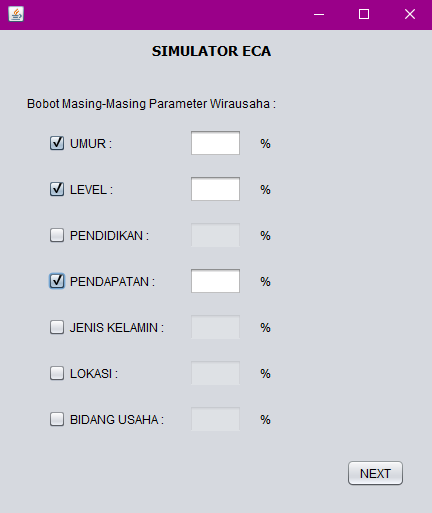
\includegraphics[width=12cm, height=13cm]{tampilanImplementasiBobot} 
		\caption[Gambar TampilanBobotKetetanggaan]{Gambar TampilanBobotKetetanggaan pada saat men-\textit{checklist checkbox}}
	\label{fig:tampilanBobot1} 
\end{figure}

	Pada saat \textit{user} sudah melakukan \textit{check list} pada \textit{checkbox}, \textit{user} harus mengisi bobot untuk setiap atribut yang telah dipilih. Total bobot atribut harus 100\%. (Gambar \ref{fig:tampilanBobot2})
	
	
	\begin{figure} [H]
	\centering  
	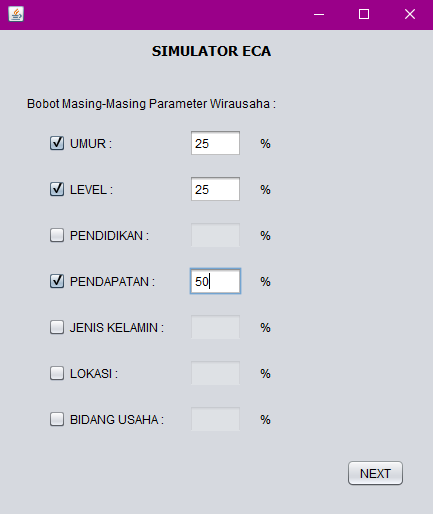
\includegraphics[width=12cm, height=13cm]{tampilanImplementasiBobot1} 
		\caption[Gambar TampilanBobotKetetanggaan]{Gambar TampilanBobotKetetanggaan pada saat mengisi bobot masing-masing atribut}
	\label{fig:tampilanBobot2} 
\end{figure}

	\item TampilanKondisiKetetanggaan
	
	Pada tampilan ini, \textit{user} diminta untuk mengisi relasi ketetanggaan pada atribut yang telah dipilih sebelumnya. (Gambar \ref{fig:tampilantetangga})
	
	\begin{figure} [H]
	\centering  
	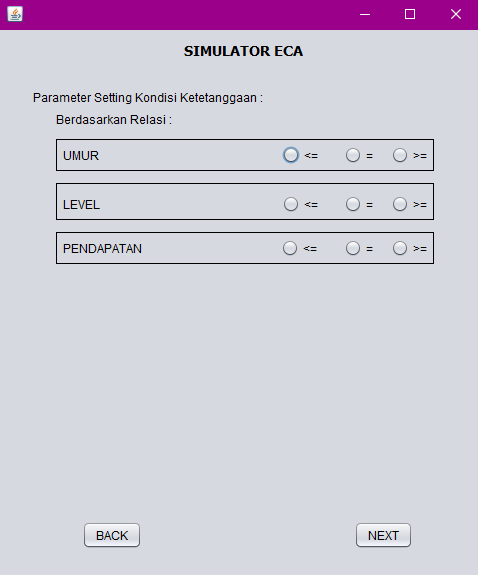
\includegraphics[width=10cm, height=12cm]{tampilanImplementasiKetetanggaan} 
		\caption[Gambar TampilanKondisiKetetanggaan]{Gambar TampilanKondisiKetetanggaan untuk atribut yang telah dipilih sebelumnya.}
	\label{fig:tampilantetangga} 
\end{figure}

	\textit{User} dapat mengisi relasi melalui \textit{radio button} dan \textit{user} hanya bisa memilih salah satu diantara tiga relasi tersebut. (Gambar \ref{fig:tampilantetangga1})
	
	\begin{figure} [H]
	\centering  
	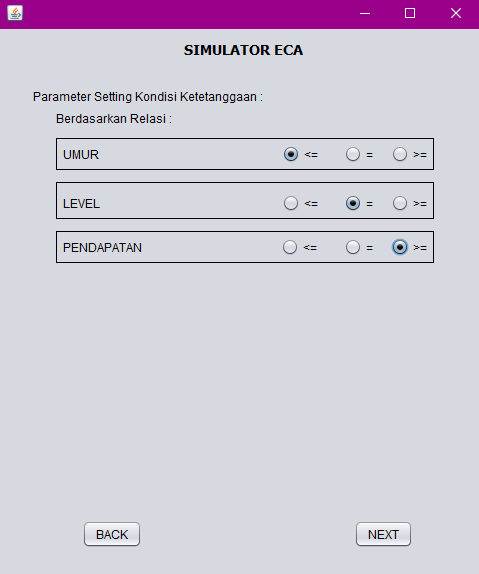
\includegraphics[width=10cm, height=12cm]{tampilanImplementasiKetetanggaan1} 
		\caption[Gambar TampilanKetetanggaan]{Gambar TampilanKondisiKetetanggaan pada saat mengisi relasi ketetanggaan}
	\label{fig:tampilantetangga1} 
\end{figure}

	\item TampilanKondisiEksternal
	
	Pada tampilan ini, \textit{user} akan mengisi bobot masing-masing faktor publik. Jumlah dari seluruh bobot harus 100\%. (Gambar \ref{fig:tampilaneksternal1})
	
		\begin{figure} [H]
	\centering  
	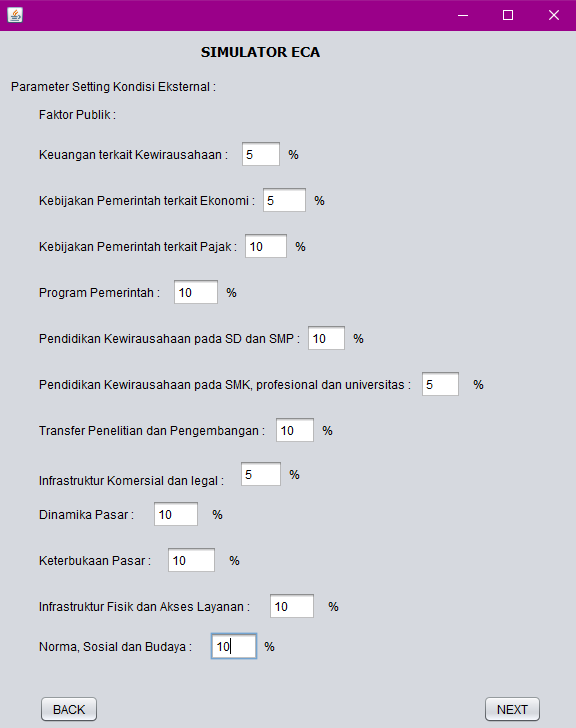
\includegraphics[width=10cm, height=12cm]{tampilanImplementasiEksternal} 
		\caption[Gambar TampilanKetetanggaan]{Gambar TampilanKondisiEksternal pada saat mengisi bobot faktor publik}
	\label{fig:tampilaneksternal1} 
\end{figure}

	\item TampilanDataWirausaha
	
 	Pada tampilan data wirausaha \textit{user} dapat meng-klik \textit{button} "OPEN FILE" yang fungsinya untuk membuka file data wirausaha yang akan disimulasikan. Data wirausaha berisi jenis kelamin, umur, usia bisnis, kategori usaha, subkategori usaha, pendidikan, lokasi, pendapatan, level dan point. Point merupakan hasil perhitungan masing-masing wirausaha pada kondisi internal. (Gambar \ref{fig:tampilandata})
	
		\begin{figure} [H]
	\centering  
	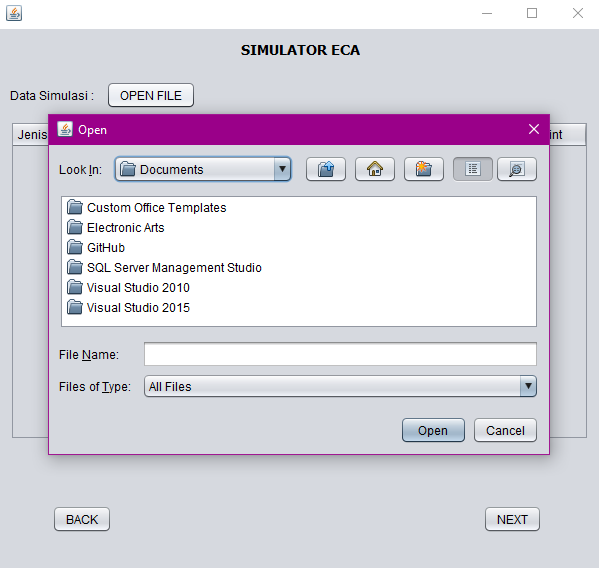
\includegraphics[width=12cm, height=12cm]{tampilanImplementasiData} 
		\caption[Gambar TampilanDataWirausaha]{Gambar TampilanDataWirausaha pada saat membuka \textit{button} "OPEN FILE"}
	\label{fig:tampilandata} 
\end{figure}

Berikut merupakan tampilan data wirausaha yang telah dipilih oleh \textit{user}. (Gambar \ref{fig:tampilandata1})
	
		\begin{figure} [H]
	\centering  
	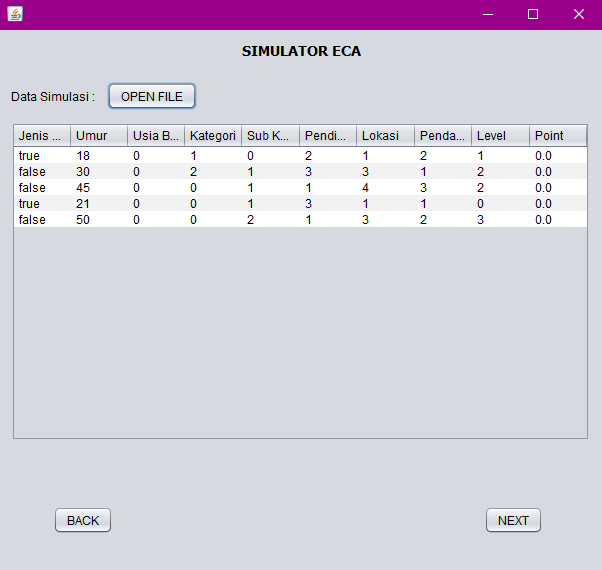
\includegraphics[width=12cm, height=12cm]{tampilanImplementasiData1} 
		\caption[Gambar TampilanDataWirausaha]{Gambar TampilanDataWirausaha saat menampilkan isi dari file}
	\label{fig:tampilandata1} 
\end{figure}

	\item TampilanSimulasi
	
	Pada tampilan ini \textit{user} diminta untuk mengisi bobot dari a,b,c,threshold dan periode. Total nilai dari a,b dan c harus 1. Setelah mengisi masing-masing nilai, \textit{user} dapat melakukan simulasi dengan cara meng-klik \textit{button} "SIMULATE".(Gambar \ref{fig:tampilansimulasi})
	
		\begin{figure} [H]
	\centering  
	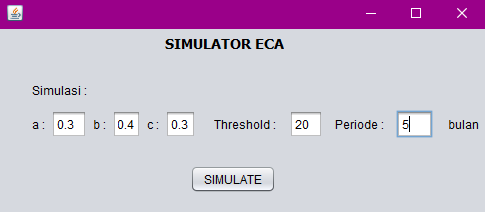
\includegraphics[width=14cm, height=8cm]{tampilanImplementasiSimulasi1} 
		\caption[Gambar TampilanSimulasi]{Gambar TampilanSimulasi pada saat mengisi bobot a,b,c,threshold dan periode}
	\label{fig:tampilansimulasi} 
\end{figure}

	\item TampilanHasil
	
	Pada tampilan ini akan ditampilkan hasil dari simulasi berupa tabel yang isi setiap kolomnya adalah iterasi (bulan), jumlah wirausaha yang berada pada level \textit{potential}, jumlah wirausaha yang berada pada level \textit{nascent}, jumlah wirausaha yang berada pada level \textit{new\_bm}, jumlah wirausaha yang berada pada level \textit{est\_bm} dan jumlah wirausaha yang berada pada level \textit{retired}. (Gambar \ref{fig:tampilanHasil})
	
	\begin{figure} [H]
	\centering  
	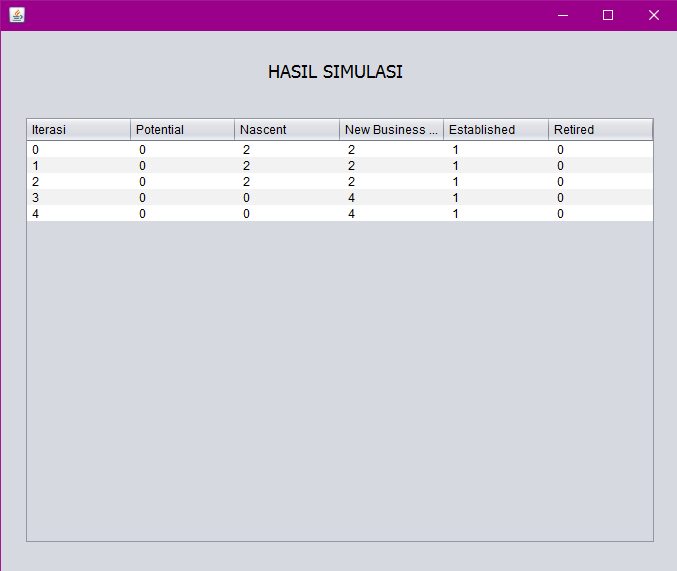
\includegraphics[width=12cm, height=10cm]{hasil2} 
		\caption[Gambar TampilanHasil]{Gambar TampilanHasil}
	\label{fig:tampilanHasil} 
\end{figure}

\end{enumerate}

\section{Pengujian}
\subsection{Pengujian Fungsional}
Pengujian fungsional dilakukan untuk mengetahui kesesuaian reaksi perangkat lunak dengan reaksi yang diharapkan berdasarkan aksi \textit{user} terhadap perangkat lunak. Pengujian ini ditujukan pada 1 pengguna yaitu \textit{user}.\\
Terdapat 8 tes kasus yang diujikan. Detail dan hasilnya dapat dilihat pada tabel \ref{tabelFungsional}

\begin{table}[H]
\centering
\caption{Tabel Pengujian Fungsional \textit{User}}
\begin{tabular}{|c|p{6cm}|p{4cm}|p{2cm}|}
\hline
No & Aksi Pengguna & Reaksi yang diharapkan & Reaksi Perangkat Lunak\\
\hline
1 & \textit{User} menjalankan simulator / aplikasi & Tampilan Bobot Ketetanggaan akan ditampilkan & Sesuai\\
\hline
2 & \textit{User} melanjutkan pengisian dengan memilih \textit{button} "NEXT" & Tampilan Kondisi Ketetanggaan akan ditampilkan & Sesuai\\
\hline
3 & \textit{User} melanjutkan pengisian dengan memilih \textit{button} "NEXT" & Tampilan Kondisi Eksternal akan ditampilkan & Sesuai\\
\hline
4 & \textit{User} melanjutkan pengisian dengan memilih \textit{button} "NEXT" & Tampilan Data Wirausaha akan ditampilkan & Sesuai\\
\hline
5 & \textit{User} memasukkan data wirausaha dengan memilih \textit{button} "OPEN FILE" & Muncul \textit{pop up windows} yang menyediakan beberapa \textit{file}, salah satu \textit{file} akan dipilih oleh \textit{user} & Sesuai\\
\hline
6 & Setelah \textit{User} memilih \textit{file} dan memilih \textit{button} "OPEN" & Data wirausaha akan ditampilkan di tabel & Sesuai\\
\hline
7 & \textit{User} melanjutkan proses simulasi dengan memilih \textit{button} "NEXT" & Tampilan Simulasi akan ditampilkan & Sesuai\\
\hline
8 & \textit{User} selesai mengisi \textit{text field} dan memilih \textit{button} "SIMULATE" & Hasil simulasi akan ditampilkan di tabel dan pada \textit{file} CSV & Sesuai\\
\hline 

\end{tabular}
\label{tabelFungsional}
\end{table} 

\subsection{Pengujian Pembacaan Parameter}
Pengujian ini dilakukan agar tidak terjadi kesalahan \textit{input} dari \textit{user} yang mengakibatkan hasil simulasi tidak sesuai dengan yang diharapkan.
\begin{enumerate}
	\item Pengisian \textit{Text Field} pada saat mengisi bobot ketetanggaan\\
	\begin{itemize}
		\item Jika \textit{user} sudah mengisi \textit{check box} tetapi tidak mengisi \textit{text field}, akan terdapat pesan kesalahan "You cannot move to the other page because you must fill text field first!". (Gambar \ref{pesanError1})
		
	\begin{figure} [H]
	\centering  
	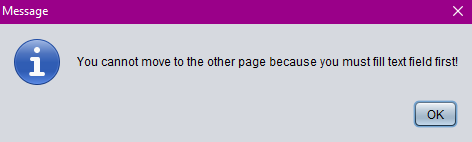
\includegraphics[width=12cm, height=4cm]{pesanError2} 
		\caption[Tampilan Pesan Error pada saat \textit{text field} tidak terisi]{Tampilan Pesan Error pada saat \textit{text field} tidak terisi}
	\label{pesanError1} 
\end{figure}
		
		\item Jika \textit{user} sudah mengisi \textit{text field} tetapi totalnya tidak 100\%, akan terdapat pesan kesalahan "The sum of text fields must 100\%!". (Gambar \ref{pesanError2})
		
	\begin{figure} [H]
	\centering  
	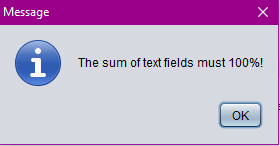
\includegraphics[width=8cm, height=4cm]{pesanError1} 
		\caption[Tampilan Pesan Error pada saat isi dari \textit{text field} tidak berjumlah 100\%]{Tampilan Pesan Error pada saat isi dari \textit{text field} tidak berjumlah 100\%}
	\label{pesanError2} 
\end{figure}

	\end{itemize}
	
	\item Pengisian \textit{Radio Button} pada saat mengisi relasi ketetanggaan\\
	Jika \textit{user} tidak mengisi radio button, akan ada pesan kesalahan yaitu "You cannot move to the other page because you must fill radio button first!". (Gambar \ref{pesanError3})
	
		\begin{figure} [H]
	\centering  
	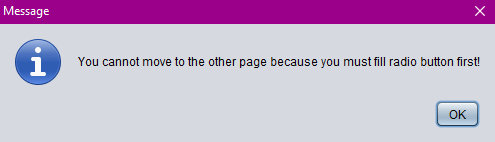
\includegraphics[width=11cm, height=4cm]{pesanError3} 
		\caption[Tampilan Pesan Error pada saat \textit{radio button} tidak terisi]{Tampilan Pesan Error pada saat \textit{radio button} tidak terisi}
	\label{pesanError3} 
\end{figure}

\item Pengisian \textit{Text Field} pada saat mengisi bobot faktor eksternal\\
	\begin{itemize}
		
		\item Jika \textit{user} tidak mengisi seluruh \textit{text field}, akan terdapat pesan kesalahan " You must fill the textfield!". (Gambar \ref{pesanError4})
		
	\begin{figure} [H]
	\centering  
	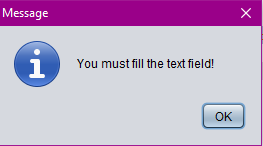
\includegraphics[width=8cm, height=4cm]{pesanError4} 
		\caption[Tampilan Pesan Error pada saat \textit{text field} tidak terisi seluruhnya]{Tampilan Pesan Error pada saat \textit{text field} tidak terisi seluruhnya}
	\label{pesanError4} 
\end{figure}
		
		\item Jika \textit{user} tidak mengisi \textit{text field}, akan terdapat pesan kesalahan "You cannot move to the other page because you must fill text field first!". (Gambar \ref{pesanError1})
		
	\begin{figure} [H]
	\centering  
	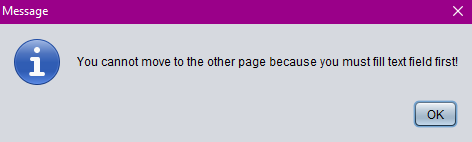
\includegraphics[width=12cm, height=4cm]{pesanError2} 
		\caption[Tampilan Pesan Error pada saat \textit{text field} tidak terisi]{Tampilan Pesan Error pada saat \textit{text field} tidak terisi}
	\label{pesanError1} 
	\end{figure}
	
	\item Jika \textit{user} sudah mengisi \textit{text field} tetapi totalnya tidak 100\%, akan terdapat pesan kesalahan "The sum of text fields must 100\%!". (Gambar \ref{pesanError2})
		
	\begin{figure} [H]
	\centering  
	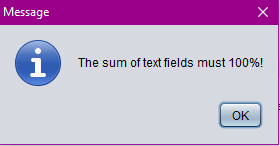
\includegraphics[width=8cm, height=4cm]{pesanError1} 
		\caption[Tampilan Pesan Error pada saat isi dari \textit{text field} tidak berjumlah 100\%]{Tampilan Pesan Error pada saat isi dari \textit{text field} tidak berjumlah 100\%}
	\label{pesanError2} 
\end{figure}
	\end{itemize}
	
	\item Pengisian nilai a,b dan c\\
	Jika \textit{user} mengisi nilai a,b dan c jumlahnya tidak 1, akan ada pesan kesalahan yaitu "The sum of a,b and c's value must 1!". (Gambar \ref{pesanError5})
	
	\begin{figure} [H]
	\centering  
	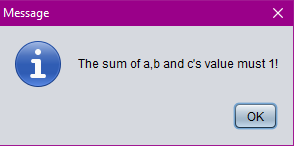
\includegraphics[width=8cm, height=4cm]{pesanError5} 
		\caption[Tampilan Pesan Error pada saat nilai a,b dan c tidak berjumlah 1]{Tampilan Pesan Error pada saat nilai a,b dan c tidak berjumlah 1}
	\label{pesanError5} 
\end{figure}
	
\end{enumerate}

\subsection{Pengujian Pembacaan File}

Pengujian pembacaan file dilakukan agar menghindari kesalahan format pada file data wirausaha yang di\textit{input} oleh \textit{user}. File tersebut untuk setiap barisnya harus berisi jenis kelamin, umur, kategori usaha, sub kategori usaha, pendidikan, lokasi, pendapatan, level wirausaha dan point.
Tipe dari masing-masing atribut yaitu :
\begin{enumerate}
	\item Jenis kelamin bertipe boolean.\\
	\begin{itemize}
		\item True untuk pria
		\item False untuk wanita
	\end{itemize}
	\item Umur bertipe bilangan bulat (dalam tahun).
	\item Kategori usaha bertipe bilangan bulat, masing-masing angka mendeskripsikan kategori usaha yang berbeda, yaitu :
		\begin{itemize}
			\item 0 untuk makanan
			\item 1 untuk minuman
			\item 2 untuk tas
			\item 3 untuk pakaian
		\end{itemize}
	\item Sub kategori usaha bertipe bilangan bulat.
		\begin{itemize}
			\item Kategori makanan :
				\begin{itemize}
					\item 0 untuk makanan ringan
					\item 1 untuk makanan berat
					\item 2 untuk makanan cepat saji
				\end{itemize}
			\item Kategori minuman :
				\begin{itemize}
					\item 0 untuk minuman sehat
					\item 1 untuk minuman bersoda
					\item 2 untuk minuman \textit{sachet}
				\end{itemize}
			\item Kategori tas :
				\begin{itemize}
					\item 0 untuk tas pria
					\item 1 untuk tas anak-anak
					\item 2 untuk tas wanita
				\end{itemize}
		\end{itemize}
		\item Pendidikan bertipe bilangan bulat, masing-masing angka mendeskripsikan tingkat pendidikan yang berbeda, yaitu :
		\begin{itemize}
					\item 0 untuk tingkat pendidikan rendah
					\item 1 untuk sekolah dasar
					\item 2 untuk sekolah menengah pertama
					\item 3 untuk sekolah menengah ke atas
					\item 4 untuk sarjana (S1)
					\item 5 untuk diploma (S2)
					\item 6 untuk profesor (S3)
				\end{itemize}
		\item Lokasi, bertipe bilangan bulat yang masing-masing angkanya mendeskripsikan lokasi yang berbeda, yaitu :
			\begin{itemize}
				\item 0 untuk Banda Aceh
				\item 1 untuk Medan
				\item 2 untuk Padang
				\item 3 untuk Pekanbaru
				\item 4 untuk Palembang
				\item 5 untuk Bandar Lampung
				\item 6 untuk Serang
				\item 7 untuk Jakarta
				\item 8 untuk Bandung
				\item 9 untuk Semarang dan Surakarta
				\item 10 untuk Surabaya
				\item 11 untuk Denpasar
				\item 12 untuk Mataram
				\item 13 untuk Kupang
				\item 14 untuk Pontianak
				\item 15 untuk Makassar
			\end{itemize}
		\item Pendapatan bertipe bilangan bulat, masing-masing angka mendeskripsikan tingkat pendapatan yang berbeda yaitu :
			\begin{itemize}
			\item 0 untuk pendapatan dibawah 3 juta rupiah
			\item 1 untuk pendapatan 3 juta rupiah sampai 5 juta rupiah
			\item 2 untuk pendapatan 5 juta rupiah sampai 7 juta rupiah
			\item 3 untuk pendapatan 7 juta rupiah sampai 9 juta rupiah
			\item 4 untuk pendapatan 9 juta rupiah sampai 11 juta rupiah
			\item 5 untuk pendapatan 11 juta rupiah sampai 13 juta rupiah
			\item 6 untuk pendapatan 13 juta rupiah sampai 15 juta rupiah
			\item 7 untuk pendapatan diatas 15 juta rupiah
			\end{itemize}
		\item Level, bertipe bilangan bulat, masing-masing angka mendeskripsikan level yang berbeda yaitu :
			\begin{itemize}
			\item 0 untuk level potential
			\item 1 untuk level nascent
			\item 2 untuk level new business manager
			\item 3 untuk level established 
			\item 4 untuk level retired
			\end{itemize}
		\item Point merupakan nilai dari kondisi internal individu wirausaha. Point mempunyai tipe data double.
\end{enumerate}

Contoh dari file data wirausaha :

	\begin{figure} [H]
	\centering  
	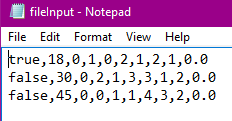
\includegraphics[width=8cm, height=4cm]{formatFile} 
		\caption[Contoh format \textit{file} data wirausaha]{Contoh format \textit{file} data wirausaha}
	\label{formatFile} 
\end{figure}

Jika \textit{user} tidak memasukkan \textit{file} data wirausaha, akan ada pesan kesalahan berupa "You must choose the file first!". (Gambar \ref{pesanError6})

	\begin{figure} [H]
	\centering  
	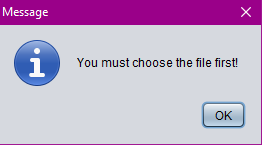
\includegraphics[width=8cm, height=4cm]{pesanError6} 
		\caption[Tampilan pesan kesalahan apabila \textit{file} data wirausaha belum dipilih]{Tampilan pesan kesalahan apabila \textit{file} data wirausaha belum dipilih}
	\label{pesanError6} 
\end{figure}

 
\subsection{Pengujian Hasil dari Simulasi}

Pengujian ini dilakukan agar hasil dari simulasi mendapatkan hasil yang akurat. Pengujian ini dilakukan dengan membandingkan hasil simulasi program dengan hasil perhitungan simulasi secara manual.\\
Contoh perhitungan menggunakan hasil perhitungan dari bab \ref{chap:analisis} pada subbab \ref{analisismodelCA}.\\
\begin{itemize}
\item Hasil Simulasi Program\\
	Berikut hasil perhitungan \textit{Continuity Index} :\\
	\begin{itemize}
		\item Iterasi pada bulan pertama
		
	\begin{figure} [H]
	\centering  
	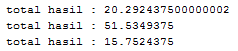
\includegraphics[width=6cm, height=3cm]{hasilIterasi0} 
		\caption[Hasil Iterasi bulan pertama]{Hasil iterasi bulan pertama}
	\label{hasilIterasi0} 
\end{figure}
		\item Iterasi pada bulan kedua
		
	\begin{figure} [H]
	\centering  
	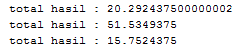
\includegraphics[width=6cm, height=3cm]{hasilIterasi1} 
		\caption[Hasil Iterasi bulan kedua]{Hasil iterasi bulan kedua}
	\label{hasilIterasi1} 
\end{figure}
		\item Iterasi pada bulan ketiga
		
	\begin{figure} [H]
	\centering  
	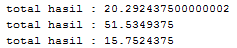
\includegraphics[width=6cm, height=3cm]{hasilIterasi2} 
		\caption[Hasil Iterasi bulan ketiga]{Hasil iterasi bulan ketiga}
	\label{hasilIterasi2} 
\end{figure}
		\item Iterasi pada bulan keempat
		
	\begin{figure} [H]
	\centering  
	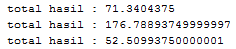
\includegraphics[width=6cm, height=3cm]{hasilIterasi3} 
		\caption[Hasil Iterasi bulan keempat]{Hasil iterasi bulan keempat}
	\label{hasilIterasi3} 
\end{figure}

		\item Iterasi pada bulan kelima
		
	\begin{figure} [H]
	\centering  
	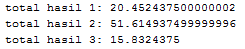
\includegraphics[width=6cm, height=3cm]{hasilIterasi4} 
		\caption[Hasil Iterasi bulan kelima]{Hasil iterasi bulan kelima}
	\label{hasilIterasi4} 
\end{figure}
		
	\end{itemize}
	Berikut hasil simulasi yang dihitung dari program : (Gambar \ref{hasil1})

	\begin{figure} [H]
	\centering  
	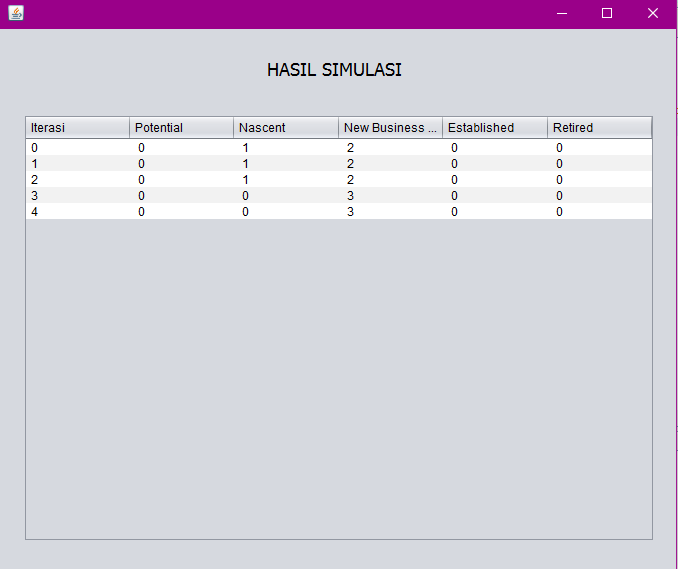
\includegraphics[width=12cm, height=10cm]{hasil1} 
		\caption[Hasil dari simulasi]{Hasil dari simulasi}
	\label{hasil1} 
\end{figure}

	Berikut rincian hasil simulasi yang ditampilkan pada Microsoft Excel (file CSV) : (Gambar \ref{hasil2})

	\begin{figure} [H]
	\centering  
	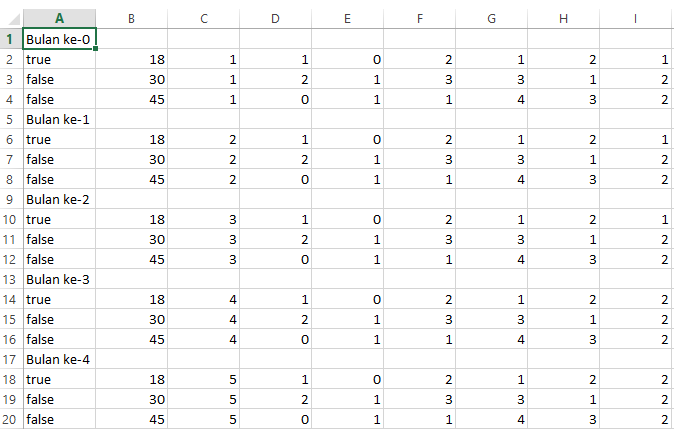
\includegraphics[width=10cm, height=8cm]{hasilExcel} 
		\caption[Hasil dari rincian simulasi]{Hasil dari rincian simulasi}
	\label{hasil2} 
\end{figure}

\item Hasil Simulasi Manual\\
Berikut hasil dari perhitungan manual :
	\begin{itemize}
		\item Iterasi pada bulan pertama
		
		\begin{multline}
	CIdx_{1}(t=0) = 0.5 \times (((14.3+4.4+19.9+11) \times 0.47) + ((14.7+17.4+5.4+10.5) \times 0.62) + ((14.3+10.4) \times 0.67)\\ + ((16+19+7.2+10.2) \times 0.8) + ((8.1+11.4) \times 0.75) + ((18.6+18.4+8.9) \times 0.35) ) + 0.4 \times (0 + 0 + 0)\\ + 0.29925 = 71.41475
\end{multline}	

\begin{multline}
	CIdx_{2}(t=0) = 0.5 \times (((29.5+49.8+2.8+41.5) \times 0.47) + ((31.6+51.5+2.4+43) \times 0.62) + ((31+41.8) \times 0.67)\\ + ((31+52+2.6+41.7) \times 0.8) + ((3.5+41.6) \times 0.75) + ((32.4+51.7 + 3.8) \times 0.35)) + 0.4 \times ((\frac {1} {2} \times 0.3) + 0 +  (\frac {1} {2} \times 0.3))\\ + 0.29925 = 176.23825
\end{multline}

\begin{multline}
	CIdx_{3}(t=0) = 0.5 \times (((17.7+17.4+1.4+2.8) \times 0.47) + ((16.1+15.4+3.1+2) \times 0.62) + ((17.6+3) \times 0.67)\\ + ((17+15+5.4+2.2) \times 0.8) + ((5.4+2.7) \times 0.75) + ((16.4+13.9) \times 0.35)) + 0.4 \times ((\frac {1} {2} \times 0.3) + 0 +  (\frac {1} {2} \times 0.3))\\ + 0.29925 = 52.08175
\end{multline}

	\item Iterasi pada bulan kedua
	
	\begin{multline}
	CIdx_{1}(t=1) = 0.5 \times (((14.3+4.4+19.9+11) \times 0.47) + ((14.7+17.4+5.4+10.5) \times 0.62) + ((14.3+10.4) \times 0.67)\\ + ((16+19+7.2+10.2) \times 0.8) + ((8.1+11.4) \times 0.75) + ((18.6+18.4+8.9) \times 0.35) ) + 0.4 \times (0 + 0 + 0)\\ + 0.29925 = 71.41475
\end{multline}	

\begin{multline}
	CIdx_{2}(t=1) = 0.5 \times (((29.5+49.8+2.8+41.5) \times 0.47) + ((31.6+51.5+2.4+43) \times 0.62) + ((31+41.8) \times 0.67)\\ + ((31+52+2.6+41.7) \times 0.8) + ((3.5+41.6) \times 0.75) + ((32.4+51.7 + 3.8) \times 0.35)) + 0.4 \times ((\frac {1} {2} \times 0.3) + 0 +  (\frac {1} {2} \times 0.3))\\ + 0.29925 = 176.23825
\end{multline}

\begin{multline}
	CIdx_{3}(t=1) = 0.5 \times (((17.7+17.4+1.4+2.8) \times 0.47) + ((16.1+15.4+3.1+2) \times 0.62) + ((17.6+3) \times 0.67)\\ + ((17+15+5.4+2.2) \times 0.8) + ((5.4+2.7) \times 0.75) + ((16.4+13.9) \times 0.35)) + 0.4 \times ((\frac {1} {2} \times 0.3) + 0 +  (\frac {1} {2} \times 0.3))\\ + 0.29925 = 52.08175
\end{multline}

	\item Iterasi pada bulan ketiga
	
	\begin{multline}
	CIdx_{1}(t=2) = 0.5 \times (((14.3+4.4+19.9+11) \times 0.47) + ((14.7+17.4+5.4+10.5) \times 0.62) + ((14.3+10.4) \times 0.67)\\ + ((16+19+7.2+10.2) \times 0.8) + ((8.1+11.4) \times 0.75) + ((18.6+18.4+8.9) \times 0.35) ) + 0.4 \times (0 + 0 + 0)\\ + 0.29925 = 71.41475
\end{multline}	

\begin{multline}
	CIdx_{2}(t=2) = 0.5 \times (((29.5+49.8+2.8+41.5) \times 0.47) + ((31.6+51.5+2.4+43) \times 0.62) + ((31+41.8) \times 0.67)\\ + ((31+52+2.6+41.7) \times 0.8) + ((3.5+41.6) \times 0.75) + ((32.4+51.7 + 3.8) \times 0.35)) + 0.4 \times ((\frac {1} {2} \times 0.3) + 0 +  (\frac {1} {2} \times 0.3))\\ + 0.29925 = 176.23825
\end{multline}

\begin{multline}
	CIdx_{3}(t=2) = 0.5 \times (((17.7+17.4+1.4+2.8) \times 0.47) + ((16.1+15.4+3.1+2) \times 0.62) + ((17.6+3) \times 0.67)\\ + ((17+15+5.4+2.2) \times 0.8) + ((5.4+2.7) \times 0.75) + ((16.4+13.9) \times 0.35)) + 0.4 \times ((\frac {1} {2} \times 0.3) + 0 +  (\frac {1} {2} \times 0.3))\\ + 0.29925 = 52.08175
\end{multline}

	\item Iterasi pada bulan keempat
	
	\begin{multline}
	CIdx_{1}(t=3) = 0.5 \times (((14.3+4.4+19.9+11) \times 0.47) + ((14.7+17.4+5.4+10.5) \times 0.62) + ((14.3+10.4) \times 0.67)\\ + ((16+19+7.2+10.2) \times 0.8) + ((8.1+11.4) \times 0.75) + ((18.6+18.4+8.9) \times 0.35) ) + 0.4 \times (0 + 0 + \frac{2}{4} \times 0.3)\\ + 0.29925 = 71.47475
\end{multline}

\begin{multline}
	CIdx_{2}(t=3) = 0.5 \times (((29.5+49.8+2.8+41.5) \times 0.47) + ((31.6+51.5+2.4+43) \times 0.62) + ((31+41.8) \times 0.67)\\ + ((31+52+2.6+41.7) \times 0.8) + ((3.5+41.6) \times 0.75) + ((32.4+51.7 + 3.8) \times 0.35)) + 0.4 \times ((\frac {1} {2} \times 0.3) + 0 +  (\frac {2} {4} \times 0.3))\\ + 0.29925 = 176.23825
\end{multline}

\begin{multline}
	CIdx_{3}(t=3) = 0.5 \times (((17.7+17.4+1.4+2.8) \times 0.47) + ((16.1+15.4+3.1+2) \times 0.62) + ((17.6+3) \times 0.67)\\ + ((17+15+5.4+2.2) \times 0.8) + ((5.4+2.7) \times 0.75) + ((16.4+13.9) \times 0.35)) + 0.4 \times ((\frac {1} {2} \times 0.3) + 0 +  (\frac {2} {4} \times 0.3))\\ + 0.29925 = 52.08175
\end{multline}

	\item Iterasi pada bulan kelima
	
	\begin{multline}
	CIdx_{1}(t=4) = 0.5 \times (((14.3+4.4+19.9+11) \times 0.47) + ((14.7+17.4+5.4+10.5) \times 0.62) + ((14.3+10.4) \times 0.67)\\ + ((16+19+7.2+10.2) \times 0.8) + ((8.1+11.4) \times 0.75) + ((18.6+18.4+8.9) \times 0.35) ) + 0.4 \times (0 + 0 + \frac{2}{4} \times 0.3)\\ + 0.29925 = 71.47475
\end{multline}

\begin{multline}
	CIdx_{2}(t=4) = 0.5 \times (((29.5+49.8+2.8+41.5) \times 0.47) + ((31.6+51.5+2.4+43) \times 0.62) + ((31+41.8) \times 0.67)\\ + ((31+52+2.6+41.7) \times 0.8) + ((3.5+41.6) \times 0.75) + ((32.4+51.7 + 3.8) \times 0.35)) + 0.4 \times ((\frac {1} {2} \times 0.3) + 0 +  (\frac {2} {4} \times 0.3))\\ + 0.29925 = 176.23825
\end{multline}

\begin{multline}
	CIdx_{3}(t=4) = 0.5 \times (((17.7+17.4+1.4+2.8) \times 0.47) + ((16.1+15.4+3.1+2) \times 0.62) + ((17.6+3) \times 0.67)\\ + ((17+15+5.4+2.2) \times 0.8) + ((5.4+2.7) \times 0.75) + ((16.4+13.9) \times 0.35)) + 0.4 \times ((\frac {1} {2} \times 0.3) + 0 +  (\frac {2} {4} \times 0.3))\\ + 0.29925 = 52.08175
\end{multline}
	\end{itemize}
\end{itemize}
